%!TEX root = ../report.tex
%%%%%%%%%%%%%%%%%%%%%%%%%%%%%%%%%%%%%%%%%%%%%%%%%%%%%%%%%%%%%%%%%%%%%%%
%%%%%%%%%%%%%%%%%%%%%%%%%%%%%%%%%%%%%%%%%%%%%%%%%%%%%%%%%%%%%%%%%%%%%%%
%%%%%                                                                 %
%%%%%     z_03_datasheet.                                             %
%%%%%                                                                 %
%%%%% Author:      Florian Zaruba                                     %
%%%%% Created:     13.12.2015                                         %
%%%%% Description: <description>                                      %
%%%%%                                                                 %
%%%%%%%%%%%%%%%%%%%%%%%%%%%%%%%%%%%%%%%%%%%%%%%%%%%%%%%%%%%%%%%%%%%%%%%
%%%%%%%%%%%%%%%%%%%%%%%%%%%%%%%%%%%%%%%%%%%%%%%%%%%%%%%%%%%%%%%%%%%%%%%

\chapter{ASIC Datasheet (Imperio)}

% If you have designed an \gls{asic} during your work, you should
% include a datasheet for your chip into the report. As soon as you
% start testing your fabricated chip, you will be glad to have such a
% datasheet. An example structure of such a datasheet is given in the
% following. For more inspirations on what you may include in your
% datasheet, have a look at the datasheet of a commercial \gls{ic}.

\minitoc

\section{Features}

\begin{itemize}
  \item RISC-V 32-bit architecture.
  \begin{itemize}
    \item 31 x 32-bit General Purpose Registers
    \item Support for RV32C and partial support for M standard extension
    \item Support for hardware loops, post incremental load and stores and SIMD packed instructions
  \end{itemize}
  \item 64 kByte RAM (32 KByte Data and Instruction)
  \item 512 kByte boot ROM
  \item Integrated FLL that offers variable speed from 0-1.2 GHz
  \item JTAG Debug Interface
  \item 19 GPIOs
  \item Peripheral Features
    \begin{itemize}
      \item Two 32-bit counter
      \item UART
      \item I2C
      \item SPI Master
      \item SPI Slave
    \end{itemize}
  \item Full scan-able design with 7 scan chains.
\end{itemize}

%\section{Applications}


\section{Description}


\section{Packaging}

A QFN40 package is used with 6 power pins.

\section{Bonding Diagram}

The extended power (ep) bonding is used for this chip. The clock pin is placed on the recommended position in order to facilitate the already manufactured tester boards in use at IIS.

\begin{figure}[htbp]
  \centering 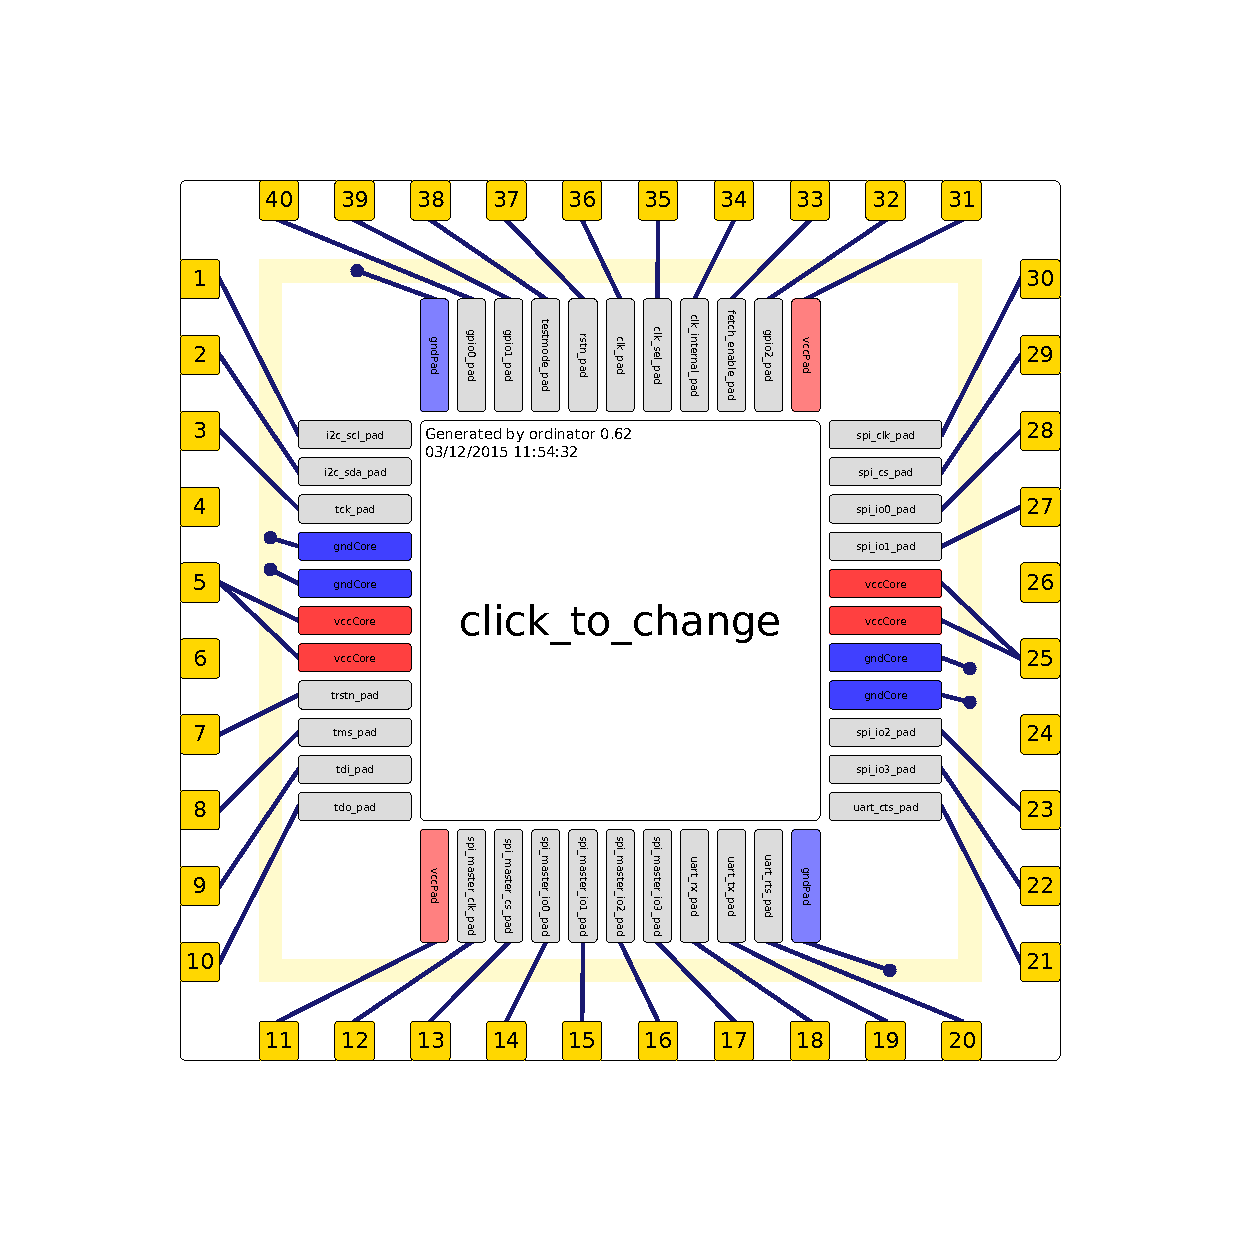
\includegraphics[width=\textwidth]{./figures/pad_instaces_img_ord}
  \caption{Bonding diagram.}
\end{figure}

\section{Pin Map}

\begin{figure}[htbp]
  \centering 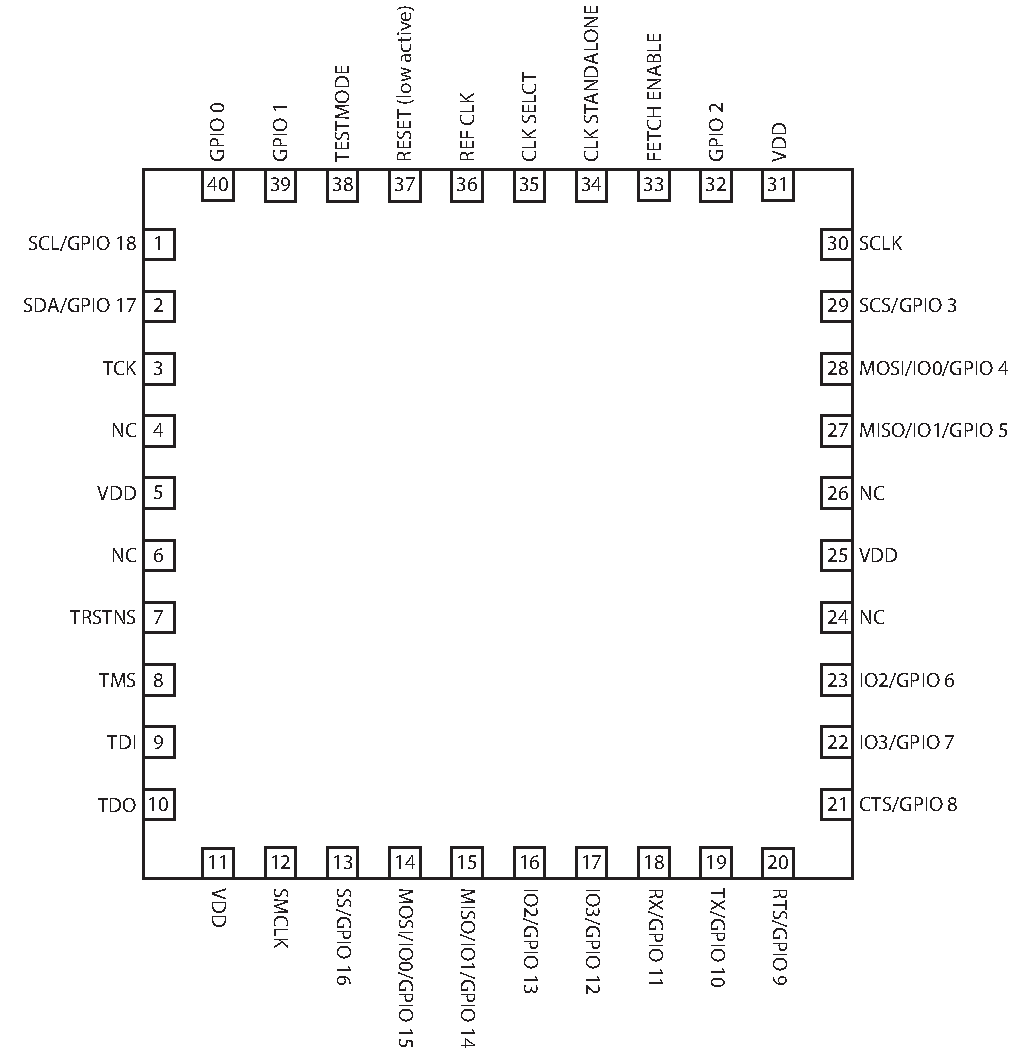
\includegraphics[width=1.0\textwidth]{./figures/pinout_imperio}
  \caption{Imperio pinout (QFN40)}
\end{figure}

\section{Pin Description}

\section{Interface Description}

\section{Register Map}

\section{Operation Modes}

\subsection{Functional Modes}
\subsection{Test Modes}

\section{Electrical Specifications}
\subsection{Recommended Operating Regions}
\subsection{Absolute Maximum Ratings}
